%%%%%%%%%%%%%%%%%%%%%%%%%%%%%%%%%%%%%%%%%
% Beamer Presentation
% LaTeX Template
% Version 1.0 (10/11/12)
%
% This template has been downloaded from:
% http://www.LaTeXTemplates.com
%
% License:
% CC BY-NC-SA 3.0 (http://creativecommons.org/licenses/by-nc-sa/3.0/)
%
%%%%%%%%%%%%%%%%%%%%%%%%%%%%%%%%%%%%%%%%%

%----------------------------------------------------------------------------------------
%	PACKAGES AND THEMES
%----------------------------------------------------------------------------------------

\documentclass[usenames,dvipsnames]{beamer}
\usepackage{xcolor}

\mode<presentation> {

% The Beamer class comes with a number of default slide themes
% which change the colors and layouts of slides. Below this is a list
% of all the themes, uncomment each in turn to see what they look like.

%\usetheme{default}
%\usetheme{AnnArbor}
%\usetheme{Antibes}
%\usetheme{Bergen}
%\usetheme{Berkeley}
%\usetheme{Berlin}
%\usetheme{Boadilla}
%\usetheme{CambridgeUS}
%\usetheme{Copenhagen}
%\usetheme{Darmstadt}
%\usetheme{Dresden}
%\usetheme{Frankfurt}
%\usetheme{Goettingen}
%\usetheme{Hannover}
%\usetheme{Ilmenau}
%\usetheme{JuanLesPins}
%\usetheme{Luebeck}
\usetheme{Madrid}
%\usetheme{Malmoe}
%\usetheme{Marburg}
%\usetheme{Montpellier}
%\usetheme{PaloAlto}
%\usetheme{Pittsburgh}
%\usetheme{Rochester}
%\usetheme{Singapore}
%\usetheme{Szeged}
%\usetheme{Warsaw}

% As well as themes, the Beamer class has a number of color themes
% for any slide theme. Uncomment each of these in turn to see how it
% changes the colors of your current slide theme.

%\usecolortheme{albatross}
\usecolortheme{beaver}
%\usecolortheme{beetle}
%\usecolortheme{crane}
%\usecolortheme{dolphin}
%\usecolortheme{dove}
%\usecolortheme{fly}
%\usecolortheme{lily}
%\usecolortheme{orchid}
%\usecolortheme{rose}
%\usecolortheme{seagull}
%\usecolortheme{seahorse}
%\usecolortheme{whale}
%\usecolortheme{wolverine}

%\setbeamertemplate{footline} % To remove the footer line in all slides uncomment this line
%\setbeamertemplate{footline}[page number] % To replace the footer line in all slides with a simple slide count uncomment this line

%\setbeamertemplate{navigation symbols}{} % To remove the navigation symbols from the bottom of all slides uncomment this line
}
\usepackage{tikz}

\usepackage{listings}
\usepackage{graphicx} % Allows including images
\usepackage{booktabs} % Allows the use of \toprule, \midrule and \bottomrule in tables
%\usepackage[T1]{fontenc}
\usepackage[utf8]{inputenc}




%----------------------------------------------------------------------------------------
%	TITLE PAGE
%----------------------------------------------------------------------------------------

\title[LINGI2142 Project 3]{LINGI2142 Computer Networks \\ Project 3} % The short title appears at the bottom of every slide, the full title is only on the title page
\titlegraphic{
\includegraphics[height=2cm]{ingi.png}}

\author[Group 2] {Group 2} % Your name
\institute[INGI] % Your institution as it will appear on the bottom of every slide, may be shorthand to save space
{
Université Catholique de Louvain - INGI\\ % Your institution for the title page
\medskip
}
\date{14st May 2014} % Date, can be changed to a custom date

%--------------------------------------
% ENVIRONMENT CUSTOMIZED
%--------------------------------------

\newenvironment{blockexample}[1]{
  \setbeamercolor{block title}{bg=OliveGreen}
  \begin{block}{Example : #1}}{\end{block}}
  
\definecolor{mygreen}{rgb}{0,0.6,0}
\definecolor{mygray}{rgb}{0.5,0.5,0.5}
\definecolor{mymauve}{rgb}{0.58,0,0.82}

\lstset{ %
  backgroundcolor=\color{white},   % choose the background color; you must add \usepackage{color} or \usepackage{xcolor}
  basicstyle=\linespread{0.40}\ttfamily\tiny,,
  breakatwhitespace=false,         % sets if automatic breaks should only happen at whitespace
  xleftmargin=5pt,
  breaklines=true,                 % sets automatic line breaking
  captionpos=b,                    % sets the caption-position to bottom
  commentstyle=\color{mygreen},    % comment style
  deletekeywords={...},            % if you want to delete keywords from the given language
  escapeinside={\%*}{*)},          % if you want to add LaTeX within your code
  extendedchars=true,              % lets you use non-ASCII characters; for 8-bits encodings only, does not work with UTF-8
  frame=single,                    % adds a frame around the code
  keepspaces=true,                 % keeps spaces in text, useful for keeping indentation of code (possibly needs columns=flexible)
  keywordstyle=\color{blue},       % keyword style
  morekeywords={*,...},            % if you want to add more keywords to the set
  numbers=left,                    % where to put the line-numbers; possible values are (none, left, right)
  numbersep=5pt,                   % how far the line-numbers are from the code
  numberstyle=\tiny\color{mygray}, % the style that is used for the line-numbers
  rulecolor=\color{black},         % if not set, the frame-color may be changed on line-breaks within not-black text (e.g. comments (green here))
  showspaces=false,                % show spaces everywhere adding particular underscores; it overrides 'showstringspaces'
  showstringspaces=false,          % underline spaces within strings only
  showtabs=false,                  % show tabs within strings adding particular underscores
  stepnumber=2,                    % the step between two line-numbers. If it's 1, each line will be numbered
  stringstyle=\color{mymauve},     % string literal style
  tabsize=2,                       % sets default tabsize to 2 spaces
%  title=\lstname                   % show the filename of files included with \lstinputlisting; also try caption instead of title
}



\begin{document}

\begin{frame}
\titlepage % Print the title page as the first slide
\end{frame}


\begin{frame}
	\tableofcontents
\end{frame}

\section*{Introduction}
\begin{frame}{\insertsection}
What we have done first : 
\begin{itemize}
\item IPV4 ? IPV6 ? 
\item Search for the addresses of the backbones routers to uses traceroutes,
\item Play with the tools on the website by trying traceroute between each destination,
\item List the differents backbones to begin a map of the network,
\item Put the cost (metrics) of each link to check if the path that we have found before are normal,
\item Tried to find the configuration of the firewall, but obviously, it was not visible,
\item Search for strange things, like: \textit{spf-delay 200};  Warning: spf-delay is deprecated
\end{itemize}
\end{frame}


\begin{frame}[fragile]{\insertsection}
\begin{lstlisting}
bgp {
	group INTERNET2 {
    	type internal;
    	local-address 64.57.28.241;
		export NEXT-HOP-SELF;
        peer-as 11537;
        inactive: neighbor 198.32.8.200 {
            description STTLng;
        }
        neighbor 64.57.28.243 {
            description ATLA;
        }
        neighbor 64.57.28.242 {
            description NEWY;
        }
        neighbor 64.57.28.244 {
            description HOUS;
        }
        neighbor 64.57.28.245 {
            description KANS;
        }
        neighbor 64.57.28.248 {
            description LOSA;
        }
        neighbor 64.57.28.246 {
            description SALT;
        }
        neighbor 64.57.28.247 {
            description SEAT;
        }
        neighbor 64.57.28.249 {
            description WASH;
        }
        neighbor 64.57.28.250 {
            description CLEV;
        }
	} 
}
\end{lstlisting}
\end{frame}





\begin{frame}{\insertsection}

Protocols found in the configuration \\

{\footnotesize
\begin{tabular}{|l|p{10cm}|}
    \hline
    \textbf{Protocols} & \textbf{Utility} \\
    \hline
    IS-IS & Used to help the backbone routers to determine the best path to reach each other.\\
    \hline
    BGP & Exchange accessibility's informations between Autonomous Systems (AS).\\
    \hline
    SNMP & Simple Network Management Protocol, used by administrator to manage network remotely.\\
    \hline
    MPLS & MultiProtocol Label Switching, mechanism to the transport of data, based on the commutation of labels that are added on the entry of the MPLS and remove at the exit.  \\
    \hline
   IGMP & Internet Group Management Protocol, permit to IP's routers to dynamically determin the multicast's groups who dispose of clients in a sub-network.\\
    \hline
    PIM & Protocol-Independent Multicast,  permit the difussion toward a group of host. \\
    \hline
    MLD & Multicast Listener Discovery, used by a router to identify the client of a multicast group on a segment directly attached. \\
    \hline
    RSVP & Permit to dynamically allocate bandwith to application oriented network.\\
    \hline
    MSDP & mechanism to connect multiple IP Version 4 Protocol Independent Multicast Sparse-Mode (PIM-SM) domains together.\\
    \hline
\end{tabular}
}
\end{frame}


\begin{frame}{\insertsection}
\begin{center} 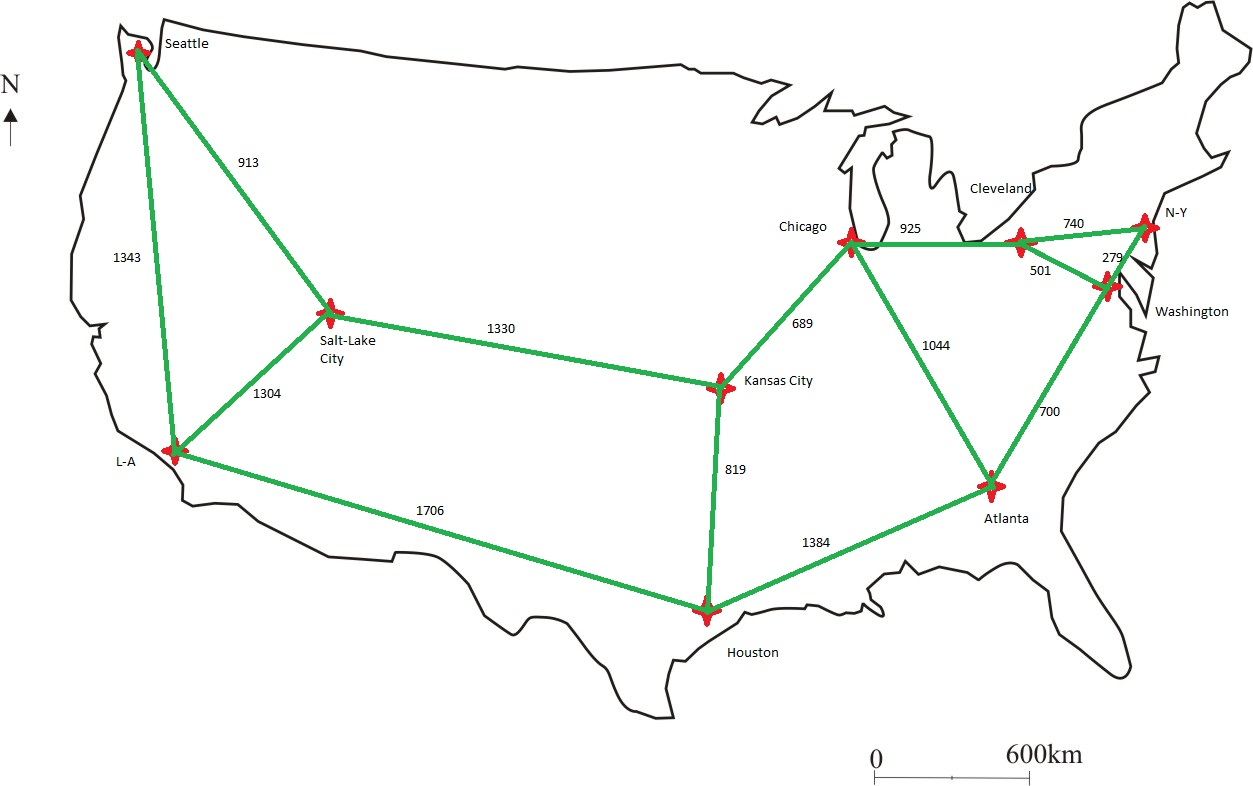
\includegraphics[scale=0.4]{map_ISIS.jpg} \end{center}
This is a map of the different backbones and routers that we deduced from the configuration.
\begin{itemize}
\item In green, the backbones links
\item In red, the backboones routers
\item In black, the "cost" of using the link to go from a router to another.
\end{itemize}
These costs are deduced thanks to the IS-IS protocol.

\end{frame}

\begin{frame}{\insertsection}
\begin{center} 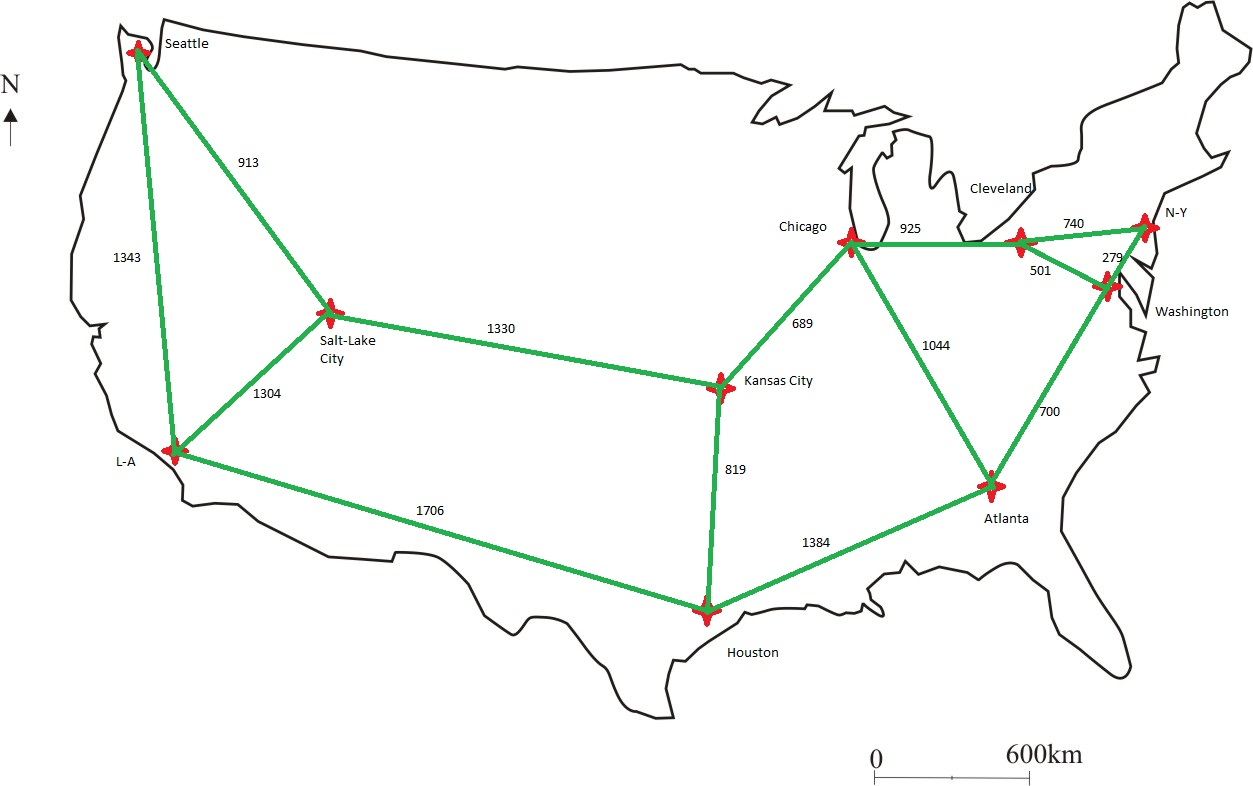
\includegraphics[width=\textwidth]{map_ISIS.jpg} \end{center}
\end{frame}



\begin{frame}{\insertsection}
\begin{center} 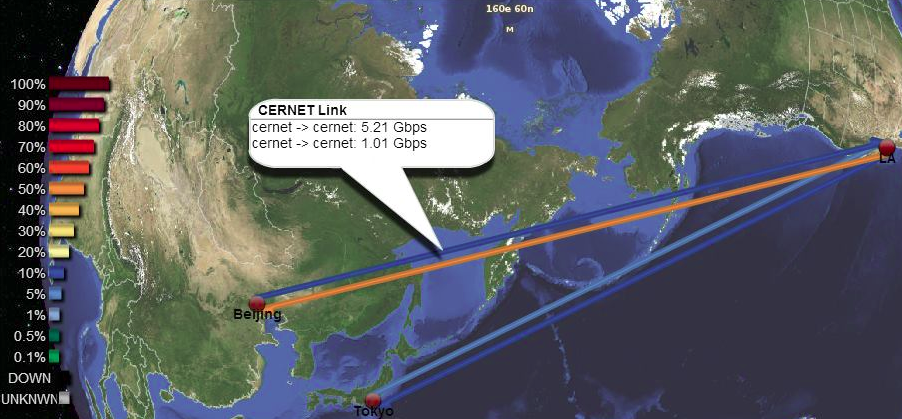
\includegraphics[width=\textwidth]{japs.png} \end{center}
On this picture, you can see that Internet2 is linked to other location in the world. We have found that when you want to access Beijing, you quit the US by L-A, for the Europa you quit the US by N-Y or Washington.We will study that later.
\end{frame}

\begin{frame}{\insertsection}
\begin{center} 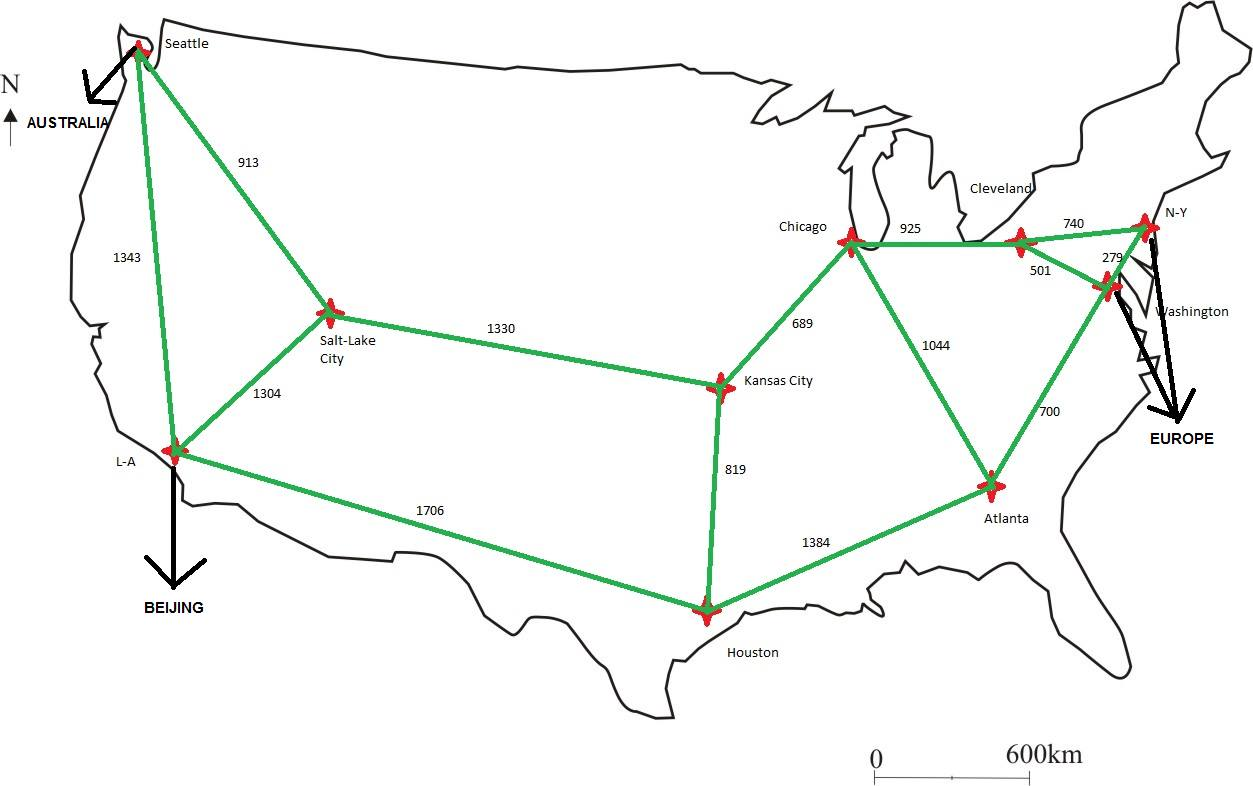
\includegraphics[width=.8\textwidth]{australie.jpg} \end{center}
On this map, you can see where the data will quit the US to reach Beijing (TransPac), Australia and Europe. Again, we have found that by using some traceroute.
\end{frame}

\section{Gateway Protocol}
\subsection{IGP}
\begin{frame}{\insertsubsection}
\begin{itemize}
  \item IS-IS protocol
  \item Find best path (Run SPF)
  \item Adjacencies - Redundancy
  \item Use ISO addresses as ID
  \item Only on Level 2 (for Backbones)
\end{itemize}
\end{frame}

\begin{frame}[fragile]{Example of IS-IS configuration}
\begin{lstlisting}[language=C]
 isis {
        export V6-IGP-AGG; /* Policy */
        no-authentication-check; /* don't reject not authenticated */
        rib-group {
            inet isis-rg;
            inet6 isis6-rg;
        }
        spf-options delay 200; /* run SPF algorithm after a network topology change */
        level 2 wide-metrics-only; /* generate metric values greater than 63 */
        /* AL2S: CLEV-NEWY R&E */
        interface et-5/0/0.102 {
            bfd-liveness-detection { /* bidirectional failure detection */ 
                minimum-interval 200; /* minimum intervals at which the local routing device transmits Hello packets */
                multiplier 3; /* number of hello packets not received to set int down */
                no-adaptation; /* not to adapt to changing network conditions */
            }
            level 1 disable;
            level 2 metric 740;
        }
}
\end{lstlisting}

\end{frame}


\subsection{Reveal eBGP peerings involving Internet2}
\begin{frame}{\insertsubsection}
\href{http://vn.grnoc.iu.edu/Internet2/bgp/bgp-summary.html}{http://vn.grnoc.iu.edu/Internet2/bgp/bgp-summary.html}\\
How can we reconstruct the BGP sessions data presented at this page ?
\end{frame}


\begin{frame}[fragile]{BGP Dump from Atlanta router from the RIB}

\begin{lstlisting}
TIME: 05/10/14 01:13:01
TYPE: TABLE_DUMP/INET
VIEW: 0
SEQUENCE: 557
PREFIX: 64.215.152.0/24
FROM:64.57.16.65 AS11537
ORIGINATED: 05/09/14 13:13:06
ORIGIN: IGP
ASPATH: 18541
NEXT_HOP: 64.57.28.248
LOCAL_PREF: 200
AGGREGATOR: AS18541 64.215.152.254
COMMUNITY: 11537:248 11537:3500 11537:5000 11537:5002 11537:5005
STATUS: 0x1
\end{lstlisting}

Conclusion : AS18541 is connected to internet2 by router 64.57.28.248 (LOSA)

\end{frame}

\subsection{Examples}

\begin{frame}[fragile]{Let's check this}
In the LOSA router configuration : 
\begin{lstlisting}[language=C]
neighbor 64.57.30.53 {
                description "[NETPLUS] I2-S10323 Blue Jeans Network";
                import [ SANITY-IN SET-PREF NETPLUS-BLUEJEANS-IN NETPLUS-CLOUD-IN ];
                export [ SANITY-OUT REMOVE-COMMS-OUT ORIGINATE4 NETPLUS-BLUEJEANS-OUT NETPLUS-CLOUD-OUT ];
                peer-as 18541;
            }
\end{lstlisting}

\end{frame}


\begin{frame}{Additionnal verifications}
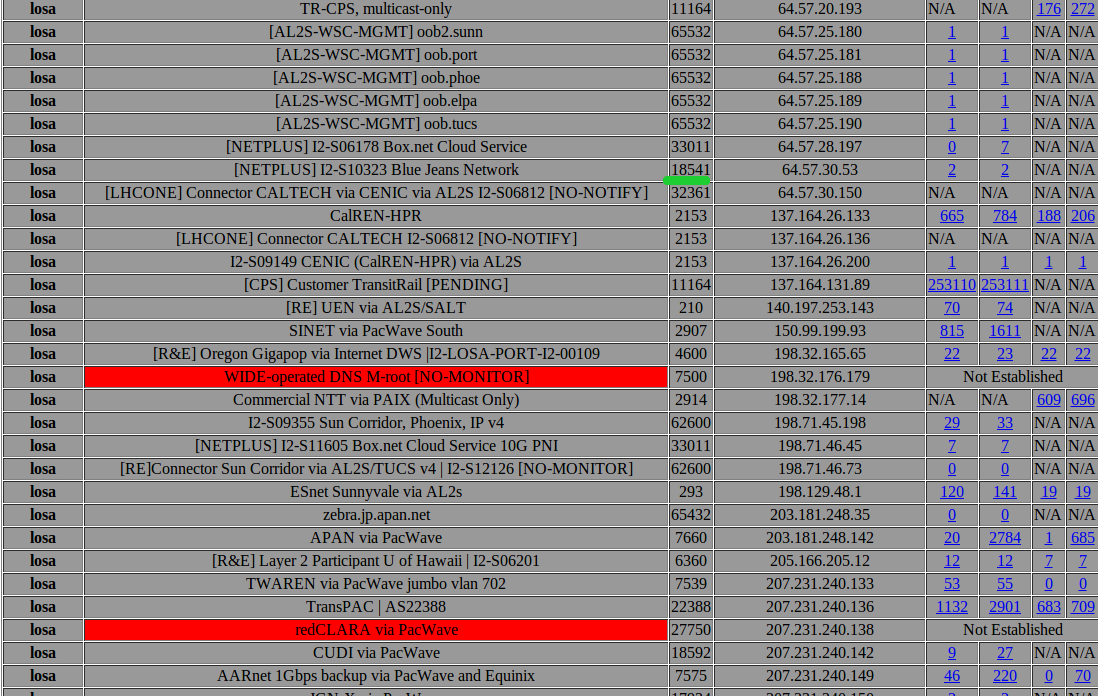
\includegraphics[width=\textwidth]{losa_18541.png}
\end{frame}

\begin{frame}{Verification from RIPE}
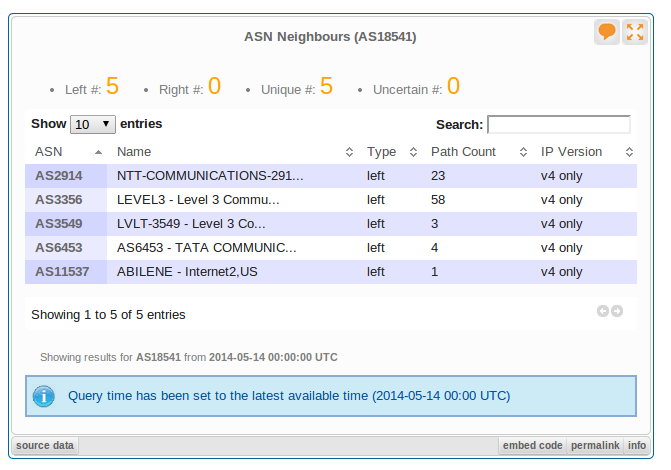
\includegraphics[width=\textwidth]{AS18541_neighbors.png}
\end{frame}

\begin{frame}[fragile]{Another Example}
\begin{lstlisting}
TIME: 05/10/14 01:13:01
TYPE: TABLE_DUMP/INET
VIEW: 0
SEQUENCE: 9482
PREFIX: 198.71.45.80/28
FROM:64.57.16.65 AS11537
ORIGINATED: 05/09/14 13:13:07
ORIGIN: IGP
ASPATH: 65532
NEXT_HOP: 64.57.25.165
MULTI_EXIT_DISC: 0
LOCAL_PREF: 100
COMMUNITY: no-export
STATUS: 0x1
\end{lstlisting}
Conclusion : AS 65532 is peer with router 64.57.25.165, which is not in the backbone, and thus corresponds to a directly connected AS.\\ Hence, Atlanta is peered with AS 65532.
\end{frame}

\begin{frame}[fragile]{Let's check this}
\begin{lstlisting}
group AL2S_MGMT {
            type external;
            metric-out igp;
            log-updown;
            import REJECT-ALL;
            family inet {
                unicast {
                    prefix-limit {
                        maximum 20;
                        teardown;
                    }
                }
            }
            export REJECT-ALL;
            remove-private;
            peer-as 65532;
            inactive: bfd-liveness-detection {
                minimum-interval 1000;
            }
            neighbor 64.57.24.204 {
                description "[AL2S-WSC-MGMT] oob.ashb";
                local-preference 300;
                hold-time 12;
                import AL2S_MGMT-IN;
            }
            ...
}
\end{lstlisting}

\end{frame}

\begin{frame}{Peering exists...}
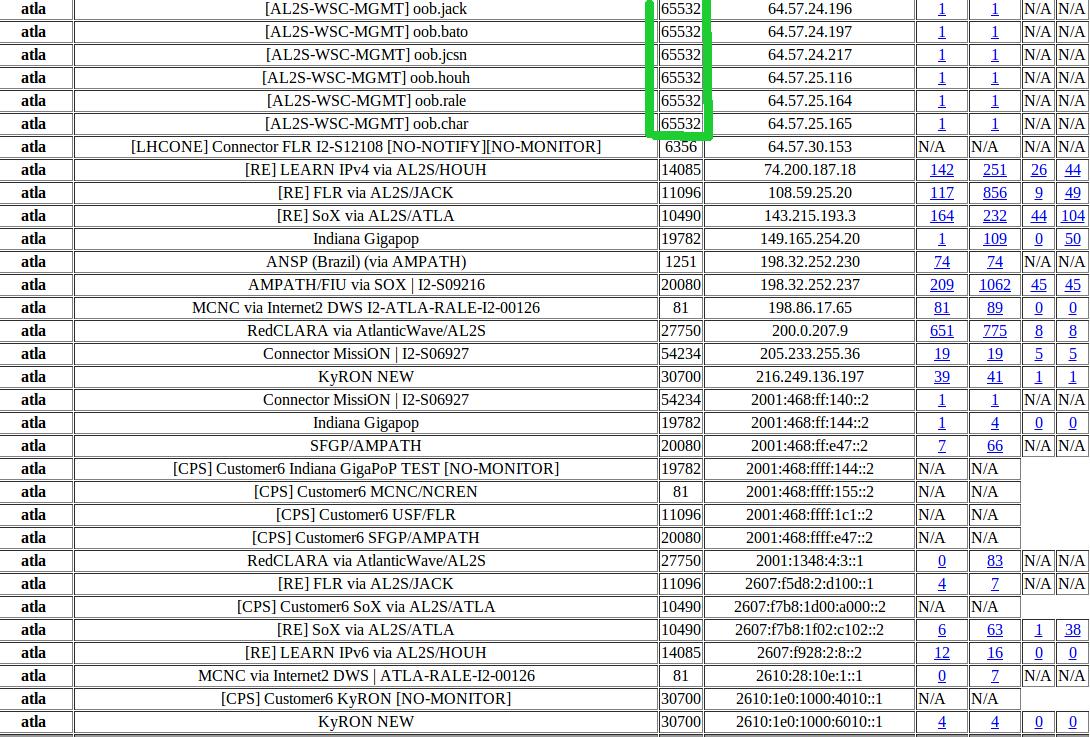
\includegraphics[width=\textwidth]{atla_65532.png}
\end{frame}


\begin{frame}{... but doesn't appear on RIPE}
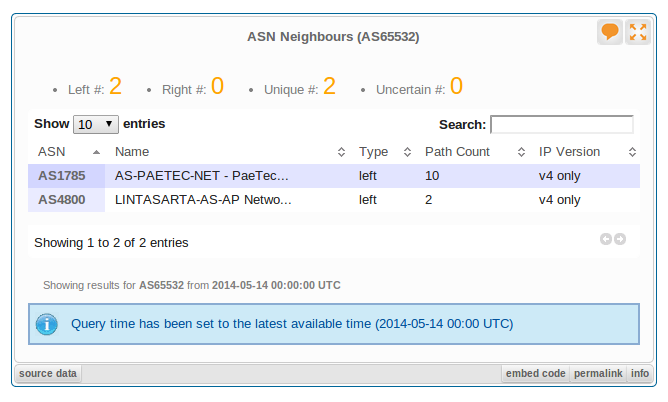
\includegraphics[width=\textwidth]{AS65532_neighbors.png}
\end{frame}

\begin{frame}[fragile]{Why ?}
\begin{lstlisting}
policy-statement AL2S_MGMT-IN {
        term accept {
            from {
                prefix-list-filter ATLA-AL2S-RACKLAN exact;
            }
            then {
                community add NO-EXPORT;
                accept;
            }
        }
        term reject {
            then reject;
        }
    }
\end{lstlisting}
\end{frame}

    


\section{MPLS}
\begin{frame}{\insertsection}
% Infer the usage of MPLS labels on data packets
% – using the mrt tool: http://www.bitwizard.nl/mtr/
% – on packets traversing Internet2 or directed to destinations in Internet2

MPLS labels:
\begin{itemize}
	\item Not visible when using MyTraceRoute (\texttt{mtr}) from outside and inside the network.
    \item But it's used according to the configuration.
\end{itemize}

\end{frame}

\subsection{Configuration}
\begin{frame}[fragile]{\insertsubsection: MPLS}
\begin{lstlisting}[language=C]
admin-groups { /* Used to include or exclude an LSP and a path's primary and secondary paths */
    r_and_e 0; /* Research and Education */
    ion 1; /* A virtual circuit network service to provide dedicated bandwidth for the most demanding apps */
}
\end{lstlisting}
\vfill
\begin{lstlisting}[language=C]
label-switched-path CHIC->SALT {
    to 64.57.28.246;
    admin-group exclude [ ion r_and_e ]; /* Exclude all members of the group */
    fast-reroute; /* Mechanism for automatically rerouting traffic on an LSP if a node or link in an LSP fails */
}
\end{lstlisting}
\vfill
\begin{lstlisting}[language=C]
label-switched-path oscars_ion_internet2_edu-11936 {
    from 64.57.28.241;
    to 64.57.28.24; /* ae-0.30.rtr.salt.net.internet2.edu: Salt-Lake */
    metric 65535; /* Compared against another LSP or against an IGP route instead of using a dynamic and automatically tracks underlying IGP metrics. */
    bandwidth 200m; /* Allocated bandwidth for the reroute path */
    priority 4 4; /* Configure the setup priority [0] and reservation priority [1] */
    primary oscars_ion_internet2_edu-11936; /* Primary path to use for an LSP */
    policing filter oscars_ion_internet2_edu-11936_policing; /* policing filter */
}
\end{lstlisting}
\vfill
\begin{lstlisting}[language=C]
path oscars_ion_internet2_edu-11936 {
    64.57.28.120 strict; /* Kans */
    64.57.28.24 strict; /* Salt */
}
\end{lstlisting}

\end{frame}

\begin{frame}[fragile]{\insertsubsection: Misc.}
We can see this previous path \texttt{oscars\_ion\_internet2\_edu-11936} in other parts of Chicago and Seattle routers:
\begin{itemize}
	\item Forwarding table (in the export section)
    \item BGP's community (example here above from Chicago configuration)
    \item Policy options (accept what come from this path and define the community)
\end{itemize}

%\begin{lstlisting}[language=C]
%policy-statement oscars_ion_internet2_edu-11936 {
%      term oscars_ion_internet2_edu-11936 {
%          from community oscars_ion_internet2_edu-11936;
%          then {
%              install-nexthop lsp oscars_ion_internet2_edu-11936;
%              accept;
%          }
%      }
%  }
%\end{lstlisting}
\begin{lstlisting}[language=C]
       neighbor 64.57.28.246 { /* Salt-Lake */
            interface xe-0/2/0.1517 {
                psn-tunnel-endpoint 64.57.28.24; /* Salt-Lake */
                virtual-circuit-id 10201517;
                description oscars_ion_internet2_edu-11936;
                community oscars_ion_internet2_edu-11936;
                mtu 9174;
            }
\end{lstlisting}

\end{frame}

\subsection{Ingress, Egress, Transit}
\begin{frame}[fragile]{\insertsubsection}
Different type of points:
\begin{itemize}
	\item Ingress point: router which encapsulates the IP packet into an MPLS packet.
    \item Egress point: router which decapsulates the IP packet from the MPLS packet.
    \item Transit router: router which simply passes the MPLS packet based on the MPLS label.
\end{itemize}

{\tiny
\hspace*{-.2cm}
\begin{tabular}{|cccccccc|}\hline
Router & Type & Name & Source & Destination & State & Lbl In & Lbl Out\\
\hline
chic & \texttt{oscars\_ion\_internet2\_edu-11936} & Ingress & 64.57.28.241 & 64.57.28.24 & Up & & \\
chic & \texttt{oscars\_ion\_internet2\_edu-11936} & Egress & 64.57.28.246 & 64.57.28.121 & Up & 3 &	- \\
kans & \texttt{oscars\_ion\_internet2\_edu-11936} & Transit & 64.57.28.241 & 64.57.28.24 & Up & 303184 & 3\\
kans & \texttt{oscars\_ion\_internet2\_edu-11936} & Transit & 64.57.28.241 & 64.57.28.24 & Up & 303184 & 3\\
salt & \texttt{oscars\_ion\_internet2\_edu-11936} & Ingress & 64.57.28.246 & 64.57.28.121 & Up & &\\
salt & \texttt{oscars\_ion\_internet2\_edu-11936} & Egress & 64.57.28.241 & 64.57.28.24 & Up & 3 & -\\
\hline
\end{tabular}
}

\end{frame}



\section{Paths and performances provided by Internet2 routers}
\subsection{First approach}
\begin{frame}[fragile]{\insertsection}
\textbf{\insertsubsection}
\vfill
First, we tried to ping addresses from loopback on each routers. Then we made the same test with some very common websites :
\begin{lstlisting}
ping count 3 google.com 
PING6(56=40+8+8 bytes) 2001:468:1::1 --> 2607:f8b0:4009:800::1004
ping: sendmsg: No route to host
ping6: wrote google.com 16 chars, ret=-1
\end{lstlisting}
\vfill
While some less common websites :
\begin{lstlisting}
ping count 3 uclouvain.be 
PING uclouvain.be (130.104.5.100): 56 data bytes
64 bytes from 130.104.5.100: icmp_seq=0 ttl=58 time=136.473 ms
\end{lstlisting}

\end{frame}


\subsection{Analysing that results}
\begin{frame}{\insertsubsection}
\begin{itemize}
\item Different user groups
	\begin{itemize}
	\item Researchers
	\item Networkers
	\item Real-time video users
	\end{itemize}
\vfill
\item Commercial peering services
	\begin{itemize}
    \item Google - Internal Gateway
    \item Amazon - aws
    \item Akamai - Computation
    \item World Bank
    \end{itemize}
\end{itemize}
\end{frame}

\begin{frame}{Inside UCL network}
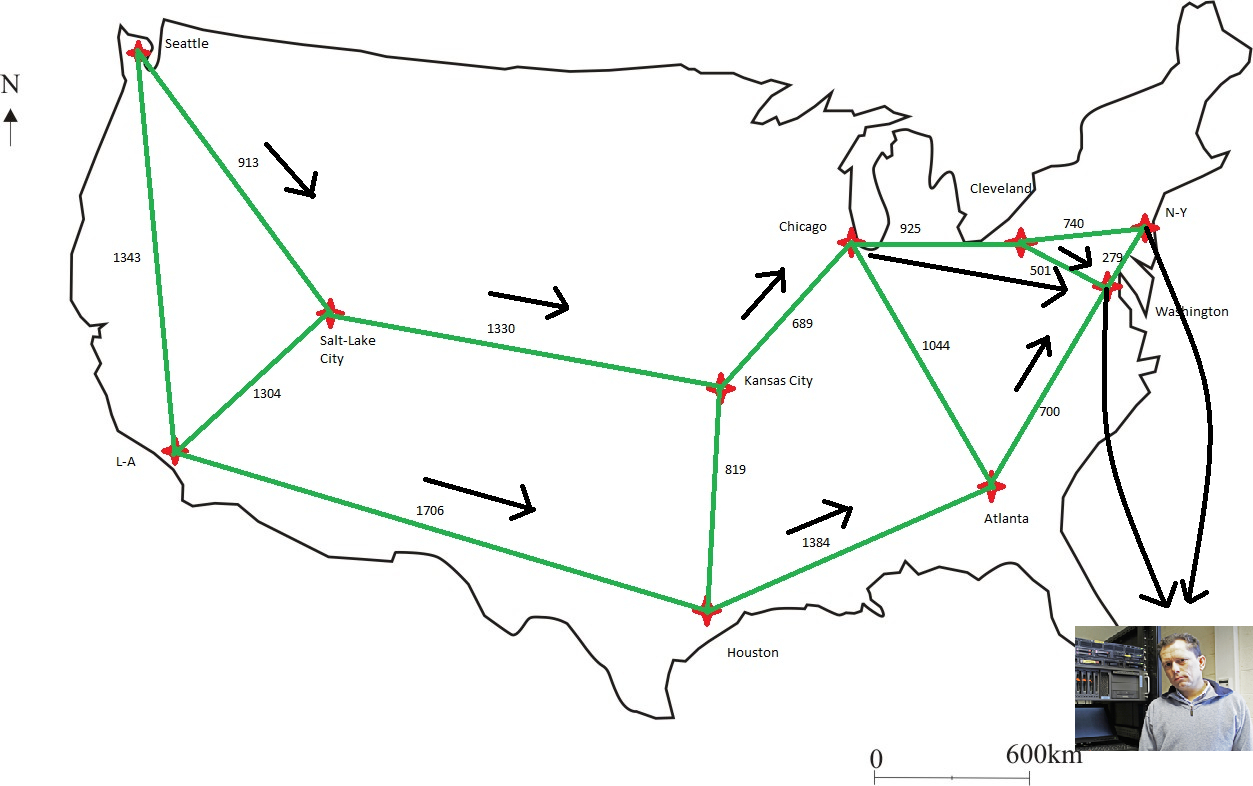
\includegraphics[width=\textwidth]{ucl_carte.png}
\end{frame}

\begin{frame}[fragile]{Inside UCL network}
\begin{lstlisting}
 traceroute 130.104.157.210 
traceroute to 130.104.157.210 (130.104.157.210), 30 hops max, 40 byte packets
 1  et-9-0-0.115.rtr.wash.net.internet2.edu (198.71.45.57)  17.700 ms  17.693 ms  17.730 ms
 2  abilene-wash.mx1.fra.de.geant.net (62.40.125.17)  111.595 ms  127.825 ms  125.481 ms
 3  ae1.mx1.ams.nl.geant.net (62.40.98.129)  122.229 ms  108.457 ms  121.801 ms
 4  xe-0-0-0.mx1.bru.be.geant.net (62.40.98.138)  125.072 ms  111.178 ms  110.951 ms
 5  belnet-gw.mx2.bru.be.geant.net (62.40.124.162)  111.168 ms  111.307 ms  111.236 ms
 6  ucl.cr2.brueve.belnet.net (193.191.3.86)  127.750 ms  126.487 ms  126.259 ms
 7  CtMichotte.sri.ucl.ac.be (130.104.254.219)  127.078 ms  127.456 ms  140.337 ms
 8  wifi-student1-3537.sri.ucl.ac.be (130.104.157.210)  156.267 ms  115.883 ms  162.040 ms

\end{lstlisting}
\end{frame}


\begin{frame}{Amazon AWS}
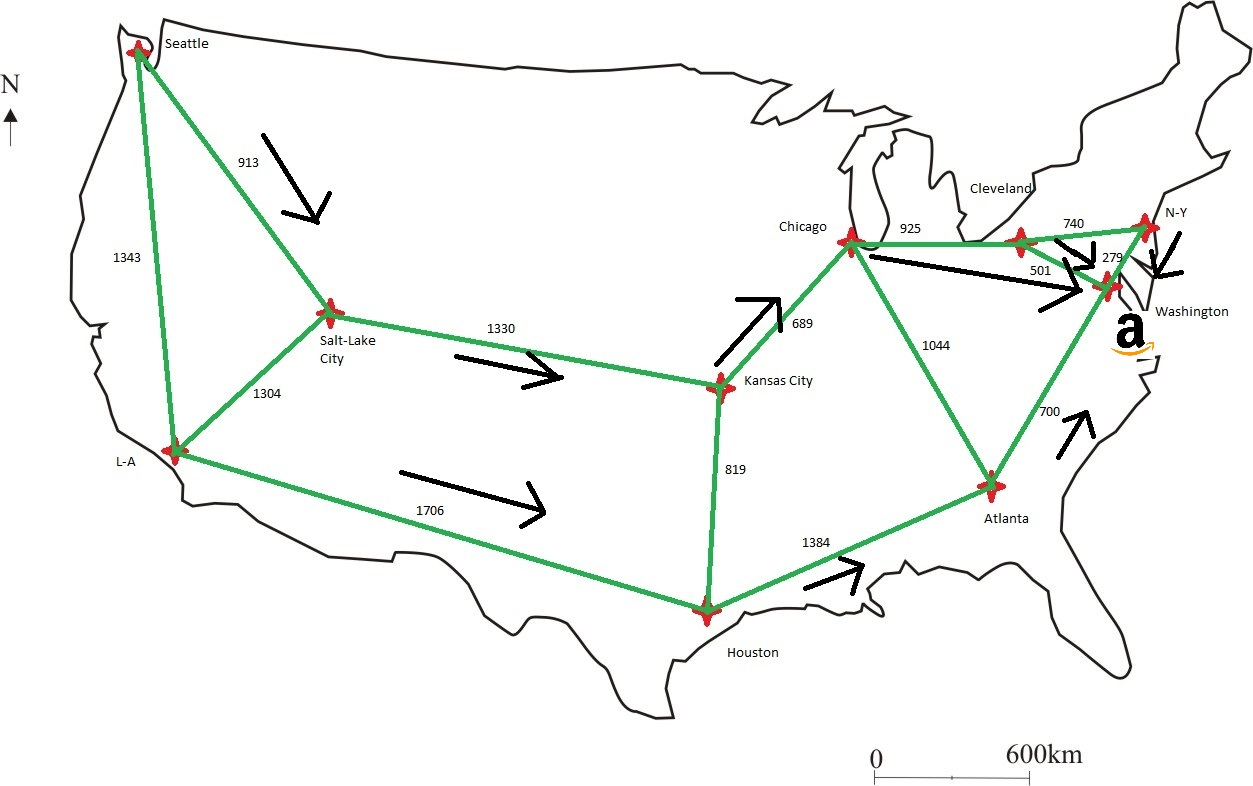
\includegraphics[width=\textwidth]{map_amazone.jpg}
\end{frame}

\begin{frame}[fragile]{Amazon AWS}
Classic from Chicago:
\begin{lstlisting}
traceroute aws.amazon.com 
traceroute to aws.amazon.com (176.32.98.131), 30 hops max, 40 byte packets
 1  et-9-0-0.115.rtr.wash.net.internet2.edu (198.71.45.57)  19.675 ms  17.736 ms  17.603 ms
 2  198.71.46.11 (198.71.46.11)  21.036 ms 198.71.46.9 (198.71.46.9)  18.396 ms 64.57.30.39 (64.57.30.39)  18.405 ms
 3  72.21.220.69 (72.21.220.69)  19.322 ms 72.21.220.37 (72.21.220.37)  18.925 ms 72.21.220.69 (72.21.220.69)  18.918 ms
     MPLS Label=403248 CoS=0 TTL=1 S=1
 4  72.21.222.35 (72.21.222.35)  19.096 ms 205.251.245.65 (205.251.245.65)  20.204 ms 72.21.222.35 (72.21.222.35)  19.409 ms
 5  * *
\end{lstlisting}
Exception on Washington:
\begin{lstlisting}
traceroute aws.amazon.com 
traceroute to aws.amazon.com (205.251.235.191), 30 hops max, 40 byte packets
 1  et-9-0-0.115.rtr.chic.net.internet2.edu (198.71.45.56)  18.321 ms  18.009 ms  39.502 ms
 2  et-10-0-0.106.rtr.kans.net.internet2.edu (198.71.45.15)  29.166 ms  28.953 ms  29.020 ms
 3  et-4-0-0.110.rtr.salt.net.internet2.edu (198.71.45.19)  49.033 ms  49.487 ms  49.405 ms
 4  et-5-0-0.113.rtr.seat.net.internet2.edu (198.71.45.25)  65.531 ms  65.381 ms  65.305 ms
 5  64.57.30.43 (64.57.30.43)  66.099 ms 64.57.30.45 (64.57.30.45)  65.246 ms 64.57.30.43 (64.57.30.43)  82.882 ms
 6  205.251.225.180 (205.251.225.180)  104.429 ms  72.816 ms 205.251.225.178 (205.251.225.178)  74.085 ms
     MPLS Label=300048 CoS=0 TTL=1 S=1
 7  205.251.232.88 (205.251.232.88)  79.369 ms 205.251.232.90 (205.251.232.90)  73.297 ms  73.015 ms
     MPLS Label=304448 CoS=0 TTL=1 S=1
 8  205.251.232.163 (205.251.232.163)  73.525 ms 205.251.232.145 (205.251.232.145)  72.985 ms 205.251.232.157 (205.251.232.157)  73.540 ms
     MPLS Label=693420 CoS=0 TTL=1 S=1
 9  205.251.230.125 (205.251.230.125)  72.696 ms  73.031 ms  73.813 ms
10  * *
\end{lstlisting}
\end{frame}


\begin{frame}{Akamai - White House}
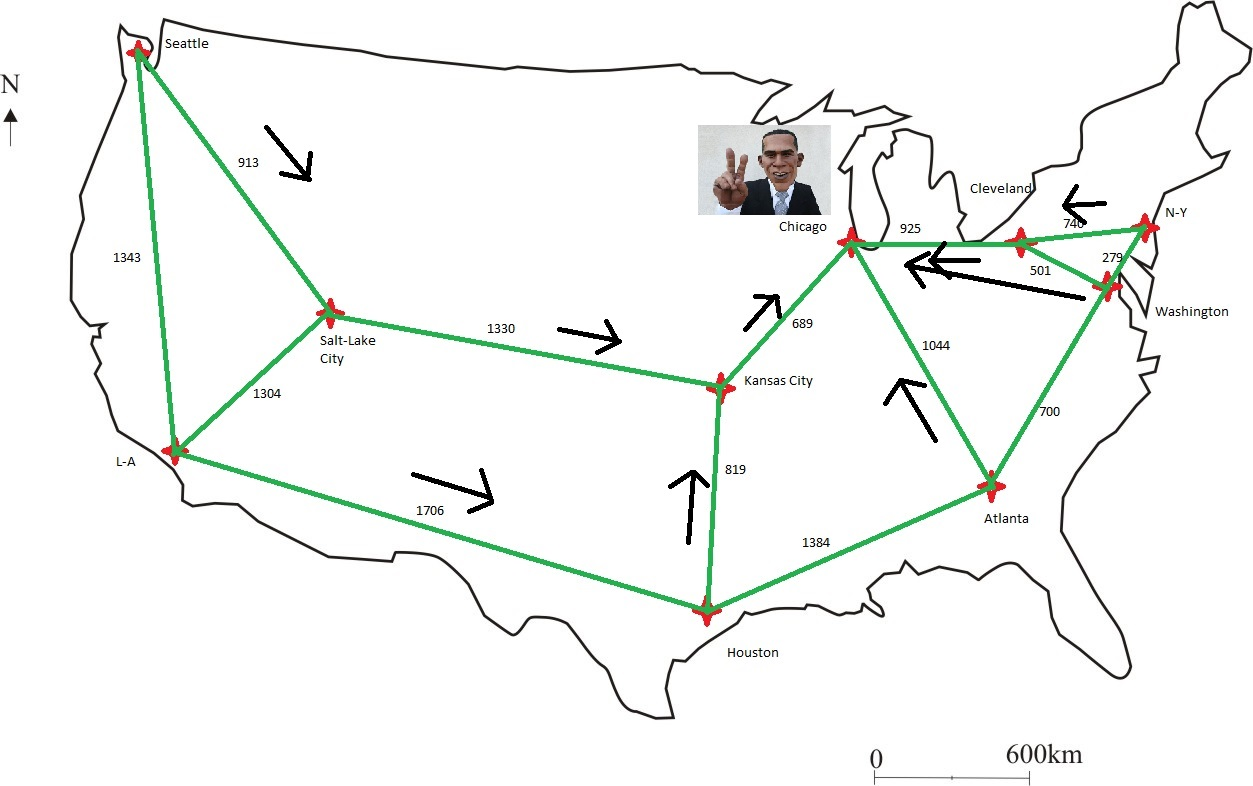
\includegraphics[width=\textwidth]{obama_carte.jpg}
\end{frame}

\begin{frame}[fragile]{Akamai - White House}
\begin{lstlisting}
traceroute www.whitehouse.gov 
traceroute6: Warning: a1128.dsch.akamai.net has multiple addresses; using 2001:18e8:2:10e::c631:b109
traceroute6 to a1128.dsch.akamai.net (2001:18e8:2:10e::c631:b109) from 2001:468:2:204::2, 64 hops max, 12 byte packets
 1  et-9-0-0.115.rtr.chic.net.internet2.edu (2001:468:2:204::1)  17.754 ms  17.925 ms  17.728 ms
 2  ae-1.2063.rtr.ictc.indiana.gigapop.net (2001:18e8:ff00::1)  22.693 ms  22.809 ms  22.356 ms
 3  ae-10.9.br2.ictc.net.uits.iu.edu (2001:18e8:ff00:2::2)  22.677 ms  22.529 ms  23.163 ms
 4  ae-0.0.br2.bldc.net.uits.iu.edu (2001:18e8:3:f002::2)  23.478 ms  23.128 ms  23.233 ms
 5  ae-10.0.dcr3.bldc.net.uits.iu.edu (2001:18e8:3:f019::2)  23.422 ms  23.692 ms  23.611 ms
 6  2001:18e8:2:10e::c631:b109 (2001:18e8:2:10e::c631:b109)  23.086 ms  23.859 ms  23.599 ms
\end{lstlisting}
\begin{itemize}
	\item www.whitehouse.gov : 2001:18e8:2:10e::c631:b108 (accessible)
    \item www.nsa.gov : 2600:1407:f:193::19ff (not accessible but found with DNS)
\end{itemize}
\end{frame}

\begin{frame}{World Bank}
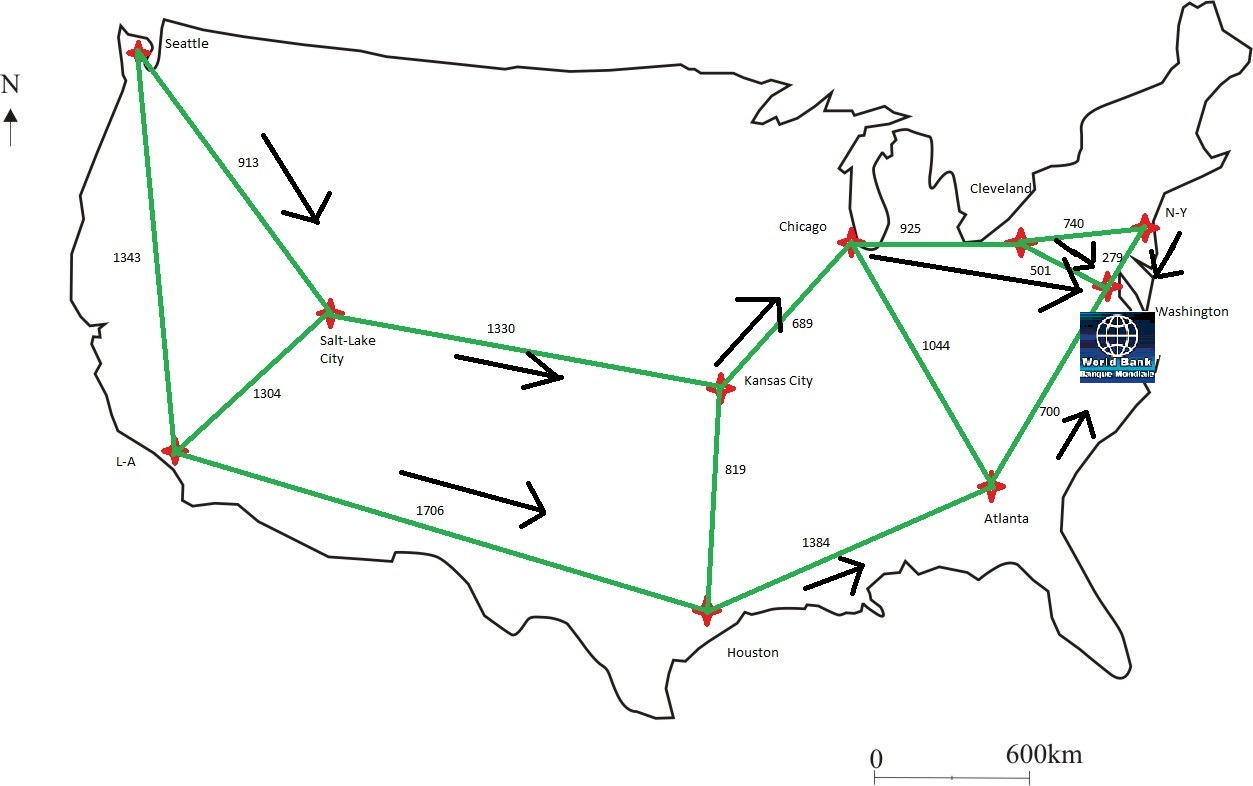
\includegraphics[width=\textwidth]{map_banque.png}
\end{frame}

\begin{frame}{Ghost Link}
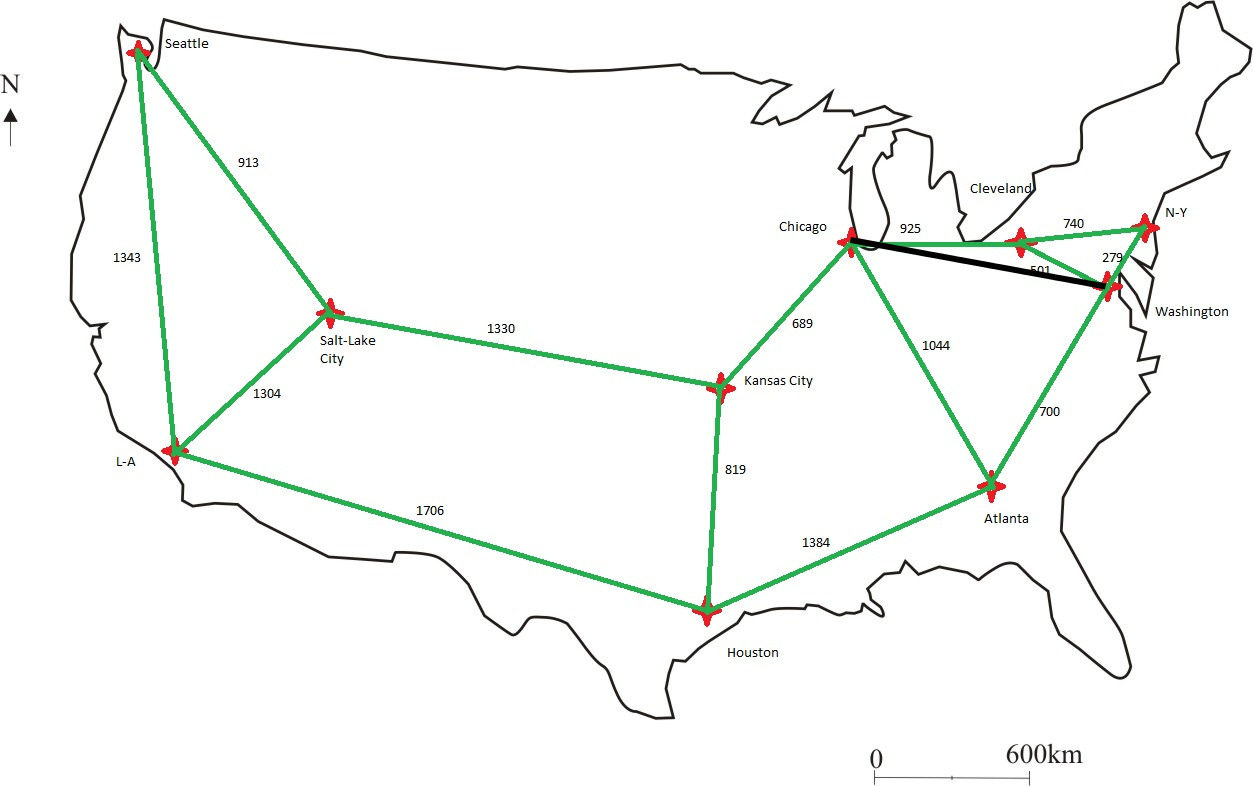
\includegraphics[width=\textwidth]{map_ghost_link.jpg}
\end{frame}


\section*{Conclusion}
\begin{frame}{\insertsection}
\begin{itemize}
	\item This project was a little fuzzy at first with these huge configuration file, but step by step it was more and more clear and finally, we finish with a good idea of the (basical) operation of this network.
	\item We have shown that the real network doesn't show exactly the same things than the configuration (or the map provided by the website), but it is just for few exceptions.
    
 \end{itemize}

\end{frame}






\end{document}